\documentclass[11pt,fleqn]{article}

\usepackage[left=34mm,right=34mm,top=45mm,bottom=60mm,centering]{geometry}
\usepackage[english]{babel}
\usepackage[utf8x]{inputenc}
\usepackage{amsmath,amssymb,amsthm}
\usepackage{graphicx}
\usepackage{mathtools}
\usepackage{bm}
\usepackage{framed}
\usepackage{hyperref}

\usepackage{tikz} 
\usetikzlibrary{arrows}

\usepackage{sectsty}
\sectionfont{\sffamily\normalsize}
\subsectionfont{\normalfont\itshape\sffamily\normalsize}
\chapterfont{\sffamily}

\newtheorem{definition}{Definition}

\newcommand{\tr}{\mathrm{tr}\,}
\newcommand{\Tr}{\mathrm{Tr}\,}
\renewcommand{\vec}[1]{\mathbf{#1}}
\renewcommand{\overline}[1]{\bar{#1}}
\renewcommand{\Re}[0]{\operatorname{Re}}
\renewcommand{\Im}[0]{\operatorname{Im}}
\renewcommand{\d}{\mathrm{d}}



\setlength\parindent{0pt}
\setlength{\parskip}{4mm plus2mm minus2mm}


\usepackage{tocloft}
\renewcommand{\cfttoctitlefont}{\sffamily\bfseries\large}
%\renewcommand{\cftchapfont}{\scshape}

\renewcommand{\cftsecfont}{\normalsize\sffamily}
%\renewcommand{\cftsecleader}{\hfill}
\renewcommand{\cftsecleader}{\cftdotfill{\cftdotsep}}
\renewcommand{\cftsecpagefont}{\cftsecfont}

\renewcommand{\cftsubsecfont}{\small\sffamily}
\renewcommand{\cftsubsecleader}{\hfill}
\renewcommand{\cftsubsecleader}{\cftdotfill{\cftdotsep}}
\renewcommand{\cftsubsecpagefont}{\cftsubsecfont}



\begin{document}

\vspace*{20mm}

{
\sffamily
\huge
\textbf{C$^\star$ boundary conditions}
\\
\rule{\textwidth}{1pt}
\\[2mm]
\large
Agostino Patella, RC$^*$ collaboration
\hfill
July 2017
}


\vspace{30mm}

%\FloatBarrier

\tableofcontents

\pagebreak



\section{Introduction}

C$^\star$ (or C-parity) boundary conditions can be chosen in the spatial directions. The \texttt{openQ*D} code allows for the following possibilities.
\begin{itemize}
   \item No C$^\star$ b.c.s in space. The gauge field satisfies periodic b.c.s, and fermions satisfy phase-periodic b.c.s.
   \item C$^\star$ b.c.s in 1 spatial direction. All fields satisfy C$^\star$ b.c.s in direction $x$, and periodic b.c.s in directions $y$ and $z$.
   \item C$^\star$ b.c.s in 2 spatial directions. All fields satisfy C$^\star$ b.c.s in directions $x$ and $y$, and periodic b.c.s in direction $z$.
   \item C$^\star$ b.c.s in 3 spatial directions. All fields satisfy C$^\star$ b.c.s in directions $x$, $y$ and $z$.
\end{itemize}
Notice that phase-periodic b.c.s for fermions are not consistent with C$^\star$ b.c.s. Boundary conditions in time can be chosen to be periodic, SF, open-SF and open. For definiteness, these notes are written having in mind periodic boundary conditions in time, unless explicitly stated otherwise. Generalization to other boundary conditions in time is straightforward and it is discussed in detail in \cite{gauge_action} (for the gauge field) and in \cite{dirac} (for the quark fields).

In \texttt{openQ*D}, C$^\star$ b.c.s are implemented by means of an orbifold construction. The global lattice is constructed by doubling the size of the $x$ direction of the physical lattice. The size of the lattice is chosen at compile time by modifying the value of the macros \texttt{L}$\mu$ and \texttt{NPROC}$\mu$ (for $\mu=0,1,2,3$) in the file \texttt{include/global.h}, as explained here.
\begin{itemize}
   \item The size of the \textit{local lattice} is $\texttt{L0} \times \texttt{L1} \times \texttt{L2} \times \texttt{L3}$.
   \item The size of the \textit{MPI-process grid} is $\texttt{NPROC0} \times \texttt{NPROC1} \times \texttt{NPROC2} \times \texttt{NPROC3}$.
   \item The size of the \textit{global lattice} is $\texttt{N0} \times \texttt{N1} \times \texttt{N2} \times \texttt{N3}$, where $\texttt{N}\mu = \texttt{L}\mu \cdot \texttt{NPROC}\mu$.
   \item The size of the \textit{physical lattice} is $\texttt{N0} \times \texttt{N1} \times \texttt{N2} \times \texttt{N3}$ if no C$^\star$ b.c.s are used, and $\texttt{N0} \times \frac{\texttt{N1}}{2} \times \texttt{N2} \times \texttt{N3}$ if C$^\star$ b.c.s are used.
\end{itemize}

In what follows, C$^\star$ b.c.s in at least one direction is assumed. The global lattice will be referred to as \textit{extended lattice}, in order to stress the fact the the direction 1 is doubled by orbifold contruction. The set of points of the extended lattice is denoted by
\begin{gather}
   \Lambda = \{ x \in \mathbb{Z}^4 \ : \ 0 \le x_\mu < N_\mu \} \ .
\end{gather}
The physical lattice $\tilde{\Lambda}$ is identified with half of the extended lattice in the following way
\begin{gather}
   \tilde{\Lambda} = \{ x \in \Lambda \ : \ x_1 < N_1/2 \} \ .
\end{gather}
The set of points $\Lambda \setminus \tilde{\Lambda}$ will be referred to as the \textit{mirror lattice}.





\section{Orbifold construction}

C$^\star$ b.c.s along direction 1 on the physical lattice are given by
\begin{subequations}
   \label{eq:orbi}
   \begin{gather}
      U(x+\tfrac{N_1}{2} \hat{1},\mu) = U(x,\mu)^* \ ,
      \label{eq:orbi:SU3} \\
      A(x+\tfrac{N_1}{2} \hat{1},\mu) = -A(x,\mu) \ ,
      \label{eq:orbi:U1} \\
      \psi(x+\tfrac{N_1}{2} \hat{1}) = C^{-1} \bar{\psi}^T(x) \ ,
      \label{eq:orbi:psi} \\
      \bar{\psi}(x+\tfrac{N_1}{2} \hat{1}) = - \psi^T(x) C \ .
      \label{eq:orbi:psibar}
   \end{gather}
\end{subequations}
The charge-conjugation matrix $C$ satisfies the following conditions
\begin{gather}
   C^T = -C \ , \qquad
   C^\dag = C^{-1} \ , \qquad
   C \gamma_\mu C^{-1} = - \gamma_\mu^T \ .
\end{gather}
On the extended lattice, points $x$ and $x + \tfrac{N_1}{2} \hat{1}$ do not coincide, so eqs.~\eqref{eq:orbi} have to be interpreted as constraints which defines the \textit{admissible} gauge and fermion fields. Eqs.~\eqref{eq:orbi} will be referred to as the \textit{orbifold constraints}.

Admissible gauge fields in the mirror lattice are completely determined by the value of the gauge field in the physical lattice via eqs.~\eqref{eq:orbi:SU3} and~\eqref{eq:orbi:U1}. The integration measure over the manifold of admissible gauge fields is given by
\begin{subequations}
   \label{eq:meas:gauge}
   \begin{gather}
      [ \d U ]_{\tilde{\Lambda}} = \prod_{\mu=0}^3 \prod_{x \in \tilde{\Lambda}} \d U(x,\mu) \ ,
      \label{eq:meas:SU3} \\
      [ \d A ]_{\tilde{\Lambda}} = \prod_{\mu=0}^3 \prod_{x \in \tilde{\Lambda}} \d A(x,\mu) \ ,
      \label{eq:meas:U1}
   \end{gather}
\end{subequations}
where the products are restricted over the physical lattice. The orbifold constraint has a slightly different meaning for fermion fields. On the physical lattice $\psi$ and $\bar{\psi}$ are independent Grassmanian variables. On the extended lattice one can choose the value of $\psi$ in each point as a complete set of independent variables. The field $\bar{\psi}$ on the extended lattice is completely determined as a function of the field $\psi$ via eqs.~\eqref{eq:orbi:psi} and~\eqref{eq:orbi:psibar}. By introducing the translation operator $T$ as
\begin{gather}
   (T \phi)(x) =
   \begin{cases}
      \phi(x + \tfrac{N_1}{2} \hat{1})  \qquad & \text{if } x \in \tilde{\Lambda} \\
      \phi(x - \tfrac{N_1}{2} \hat{1})  \qquad & \text{if } x \in \Lambda \setminus \tilde{\Lambda}
   \end{cases}
   \ ,
\end{gather}
the relation between $\psi$ and $\bar{\psi}$ can be conveniently rewritten as
\begin{gather}
   \bar{\psi} = - \psi^T C T \ .
   \label{eq:majorana}
\end{gather}
The integration measure for the fermion field is given by
\begin{gather}
   [ \d \psi ]_{\tilde{\Lambda}} [ \d \bar{\psi} ]_{\tilde{\Lambda}}
   =
   \prod_{x \in \tilde{\Lambda}} \d \psi(x) \d \bar{\psi}(x)
   =
   \prod_{x \in \Lambda} \d \psi(x)
   =
   [ \d \psi ]_\Lambda
   \ .
   \label{eq:meas:fermion}
\end{gather}

Since the square of the charge-conjugation operation is the identity, all fields must obey periodic boundary conditions along the extended direction 1, i.e.
\begin{subequations}
   \label{eq:periodic}
   \begin{gather}
      U(x+N_1 \hat{1},\mu) = U(x,\mu) \ ,
      \label{eq:periodic:SU3} \\
      A(x+N_1 \hat{1},\mu) = A(x,\mu) \ ,
      \label{eq:periodic:U1} \\
      \psi(x+N_1 \hat{1}) = \psi(x) \ ,
      \label{eq:periodic:psi} \\
      \bar{\psi}(x+N_1 \hat{1}) = \bar{\psi}(x) \ .
      \label{eq:periodic:psibar}
   \end{gather}
\end{subequations}
C$^\star$ b.c.s in directions $k=2,3$ are implemented by modifying the global geometry of the torus. If $k=2,3$ is a C$^\star$ direction, then shifted boundary conditions (see fig.~\ref{fig:shifted-bc}) are imposed
\begin{subequations}
   \label{eq:shifted}
   \begin{gather}
      U(x + N_k \hat{k},\mu) = U(x+\tfrac{N_1}{2} \hat{1},\mu) \ ,
      \label{eq:shifted:SU3} \\
      A(x + N_k \hat{k},\mu) = A(x+\tfrac{N_1}{2} \hat{1},\mu) \ ,
      \label{eq:shifted:U1} \\
      \psi(x + N_k \hat{k}) = \psi(x+\tfrac{N_1}{2} \hat{1}) \ ,
      \label{eq:shifted:psi} \\
      \bar{\psi}(x + N_k \hat{k}) = \bar{\psi}(x+\tfrac{N_1}{2} \hat{1}) \ .
      \label{eq:shifted:bar}
   \end{gather}
\end{subequations}
When combined with the orbifold constraint~\eqref{eq:orbi}, shifted b.c.s are equivalent to C$^\star$ b.c.s. in direction $k=2,3$. For instance for the SU(3) gauge field,
\begin{gather}
   U(x + N_k \hat{k},\mu) = U(x+\tfrac{N_1}{2} \hat{1},\mu) = U(x,\mu)^* \ .
\end{gather}



\begin{figure}

\centering

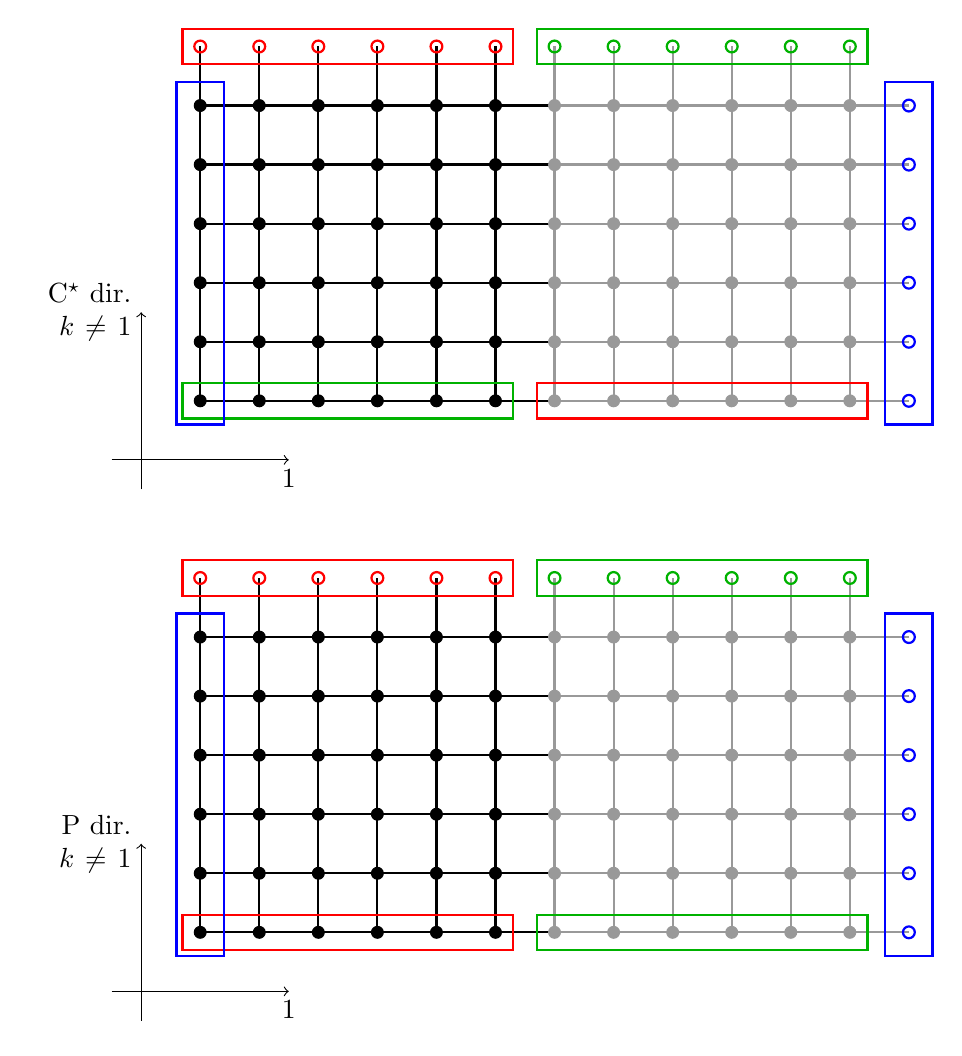
\begin{tikzpicture}[scale=.75]

   \draw[->] (-1.5,-1) -- ++(3,0) node[anchor=north] {1};
   \draw[->] (-1,-1.5) -- ++(0,3) node[anchor=east,text width=12mm,align=right] {C$^\star$ dir.\\$k \neq 1$};
   
   \foreach \x in {0,1,...,5} {
      \foreach \y in {0,1,...,5} {
         \draw[fill=black] (\x,\y) circle (.1);
         \draw[thick] (\x,\y) -- ++(1,0);
         \draw[thick] (\x,\y) -- ++(0,1);
      }
   }
   \foreach \x in {6,7,...,11} {
      \foreach \y in {0,1,...,5} {
         \draw[black!40,fill=black!40] (\x,\y) circle (.1);
         \draw[thick,black!40] (\x,\y) -- ++(1,0);
         \draw[thick,black!40] (\x,\y) -- ++(0,1);
      }
   }
   
   \foreach \x in {0,1,...,5} {
      \draw[red,thick] (\x,6) circle (.1);
   }
   \draw[red,thick] (-.3,5.7) rectangle (5.3,6.3);
   \draw[red,thick] (5.7,-.3) rectangle (11.3,.3);
   
   \foreach \x in {6,7,...,11} {
      \draw[green!70!black,thick] (\x,6) circle (.1);
   }
   \draw[green!70!black,thick] (5.7,5.7) rectangle (11.3,6.3);
   \draw[green!70!black,thick] (-.3,-.3) rectangle (5.3,.3);
   
   \foreach \y in {0,1,...,5} {
      \draw[blue,thick] (12,\y) circle (.1);
   }
   \draw[blue,thick] (11.6,-.4) rectangle (12.4,5.4);
   \draw[blue,thick] (-.4,-.4) rectangle (.4,5.4);
   
   \begin{scope}[yshift=-9cm]
      \draw[->] (-1.5,-1) -- ++(3,0) node[anchor=north] {1};
      \draw[->] (-1,-1.5) -- ++(0,3) node[anchor=east,text width=12mm,align=right] {P dir.\\$k \neq 1$};
      
      \foreach \x in {0,1,...,5} {
         \foreach \y in {0,1,...,5} {
            \draw[fill=black] (\x,\y) circle (.1);
            \draw[thick] (\x,\y) -- ++(1,0);
            \draw[thick] (\x,\y) -- ++(0,1);
         }
      }
      \foreach \x in {6,7,...,11} {
         \foreach \y in {0,1,...,5} {
            \draw[black!40,fill=black!40] (\x,\y) circle (.1);
            \draw[thick,black!40] (\x,\y) -- ++(1,0);
            \draw[thick,black!40] (\x,\y) -- ++(0,1);
         }
      }
      
      \foreach \x in {0,1,...,5} {
         \draw[red,thick] (\x,6) circle (.1);
      }
      \draw[red,thick] (-.3,5.7) rectangle (5.3,6.3);
      \draw[red,thick] (-.3,-.3) rectangle (5.3,.3);
      
      \foreach \x in {6,7,...,11} {
         \draw[green!70!black,thick] (\x,6) circle (.1);
      }
      \draw[green!70!black,thick] (5.7,5.7) rectangle (11.3,6.3);
      \draw[green!70!black,thick] (5.7,-.3) rectangle (11.3,.3);
      
      \foreach \y in {0,1,...,5} {
         \draw[blue,thick] (12,\y) circle (.1);
      }
      \draw[blue,thick] (11.6,-.4) rectangle (12.4,5.4);
      \draw[blue,thick] (-.4,-.4) rectangle (.4,5.4);
   \end{scope}
   
\end{tikzpicture}

\caption{\small\textbf{Global geometry of extended lattice.} The \textit{top diagram} represents a section of the extended lattice $\Lambda$ along a $(1,k)$ plane where $k=2,3$ is a C$^\star$ direction. All fields are periodic along the extended direction 1. C$^\star$ boundary conditions in the direction $k=2,3$ are replaced by shifted boundary conditions in the extended lattice. Shifted boundary conditions are imposed by properly defining the nearest neighbours of boundary sites. Empty circles in the red (resp. green, blue) rectangle have to be identified with the corresponding solid circles in the red (resp. green, blue) rectangle. The \textit{bottom diagram} represents a section of the extended lattice $\Lambda$ along a $(1,k)$ plane where $k=2,3$ is a periodic direction. In \textit{both diagrams}, the black circles represent the sites of the physical lattice, and the grey circles represent the sites of the mirror lattice.
\label{fig:shifted-bc}
}

\end{figure}




\section{Gauge action}

Let $\mathcal{S}_0$ and $\mathcal{S}_1$ be the sets of oriented plaquette and double-plaquette loops on the extended lattice $\Lambda$. Summing over all plaquette and double-plaquette loops in the extended lattice instead of the physical lattice introduces a double counting which can be corrected with an extra $1/2$ factor in the gauge actions:
\begin{gather}
   S_{\text{G,SU(3)}} = \frac{1}{2g_0^2} \sum_{k=0}^1 c^\text{SU(3)}_k \sum_{\mathcal{C} \in \mathcal{S}_k} w^\text{SU(3)}_k(\mathcal{C}) \ \tr [ 1 - U(\mathcal{C}) ] \ ,
   \label{eq:action:SU3} \\
   S_{\text{G,U(1)}} = \frac{1}{4 q_\text{el}^2 e_0^2} \sum_{k=0}^1 c^\text{U(1)}_k \sum_{\mathcal{C} \in \mathcal{S}_k} w^\text{U(1)}_k(\mathcal{C}) \ [ 1 - z(\mathcal{C}) ] \ ,
   \label{eq:action:U1}
\end{gather}
where $U(\mathcal{C})$ and $z(\mathcal{C})$ are the SU(3) and U(1) parallel transports along the path $\mathcal{C}$, the coefficient $c_{0,1}$ satisfy the relation
\begin{gather}
   c_0 + 8c_1 = 1 \ ,
\end{gather}
and the weight factors $w_k(\mathcal{C})$ depend on the time boundary conditions, and are different from one only close to the boundaries (see \cite{gauge_action} for more details).



\section{Dirac operator and (pseudo)fermion action}

Let $D[U,z]$ be the Dirac operator defined on the extended lattice, defined with periodic boundary conditions in direction 1, and possibly shifted boundary condition in directions $k=2,3$. When not needed, the dependence on the gauge fields $U$ and $z = e^{iA}$ will be understood. An explicit expression for the Dirac operator can be found in \cite{dirac}.

The sum over the extended lattice introduces a double counting which can be corrected with an extra $1/2$ factor in the fermion action:
\begin{gather}
   S_\text{f} = \frac{1}{2} \sum_{x \in \Lambda} \bar{\psi}(x) D \psi(x) = - \frac{1}{2} \sum_{x \in \Lambda} \psi(x)^T C T D \psi(x) \equiv -\frac{1}{2} \psi^T CTD \psi \ ,
\end{gather}
where the orbifold constraint~\eqref{eq:majorana} has been used. By using the properties of the $C$ matrix one easily proves that
\begin{gather}
   D[U,z]^T = C D[U^*,z^*] C^{-1} \ .
\end{gather}
If the gauge field respects the orbifold constraint, one trivially gets
\begin{gather}
   T D[U^*,z^*] T^{-1} = D[U,z] \ .
\end{gather}
By combining the previous two equations, and by using the fact that $C$ is anti-symmetric while $T$ is symmetric, one gets that the matrix $CTD$ is anti-symmetric
\begin{gather}
   (CTD[U,z])^T = - CTD[U,z] \ .
\end{gather}
The integration over the fermion field yields the Pfaffian of $CTD$ up to an irrelevant overall factor which will be reabsorbed in the definition of the fermionic integration measure,
\begin{gather}
   \int [ \d \psi ]_\Lambda e^{- S_f} = \int [ \d \psi ]_\Lambda e^{\frac{1}{2} \psi^T CTD \psi} = \text{Pf}\, (CTD) \ .
\end{gather}

In the continuum limit, the Pfaffian of $CTD$ is positive \cite{Lucini:2015hfa}. However at fixed lattice spacing, the Pfaffian is shown to be real but it can be negative on rough enough gauge configurations. The absolute value of the Pfaffian of $CTD$ has a representation in terms of a pseudofermion action (notice that $\det C = \det T = 1$),
\begin{gather}
   | \text{Pf}\, (CTD) | = | \text{Det}\, (CTD) |^{1/2} = \text{Det}\, (D^\dag D)^{1/4}
   =
   \int [\d \phi]_\Lambda [\d \phi^*]_\Lambda \ e^{-S_\text{pf}} \ , \\
   S_\text{pf}
   =
   \sum_{x \in \Lambda} \phi(x)^\dag (D^\dag D)^{-1/4} \phi(x)
   \equiv
   \phi^\dag (D^\dag D)^{-1/4} \phi
   \ .
\end{gather}
The pseudofermion $\phi$ is a complex field with gauge and spinor indices. It satisfies periodic boundary conditions in direction 1, and possibly shifted boundary condition in directions $k=2,3$. It is completely unrestricted over the extended lattice.

In practice even-odd preconditioning can be used, and the inverse fourth root can be replaced by a rational approximation.



\section{Molecular dynamics}

The momentum fields associated to the SU(3) and U(1) gauge fields are denoted by $\Pi(x,\mu)$ and $\pi(x,\mu)$ respectively. The momentum $\Pi(x,\mu)$ lives in the Lie algebra of SU(3),
\begin{gather}
   \Pi(x,\mu) = \Pi^a(x,\mu) T^a \ ,
\end{gather}
where $\Pi^a(x,\mu)$ are taken to be real. The momentum field $\pi(x,\mu)$ is taken to be real, like the gauge field $A(x,\mu)$. Without C$^\star$ b.c.s, the molecular dynamics (MD) Hamiltonian and the forces implemented in \texttt{openQ*D} are described in \cite{rhmc}.

With C$^\star$ b.c.s, the momentum fields must satisfy the orbifold constraint
\begin{subequations}
   \label{eq:orbi:mom}
   \begin{gather}
      \Pi(x+\tfrac{N_1}{2} \hat{1},\mu) = \Pi(x,\mu)^* \ ,
      \label{eq:orbi:momSU3} \\
      \pi(x+\tfrac{N_1}{2} \hat{1},\mu) = -\pi(x,\mu) \ .
      \label{eq:orbi:momU1}
   \end{gather}
\end{subequations}
Summing over all momenta in the extended lattice instead of the physical lattice introduces a double counting which can be corrected with an extra $1/2$ factor in the MD Hamiltonian:
\begin{gather}
   H = \frac{1}{4} \sum_{x,\mu} \bigg\{ [\pi(x,\mu)]^2 + \sum_a [\Pi^a(x,\mu)]^2 \bigg\} + S(U,A) \ .
\end{gather}

In deriving the MD equations, one needs to take into account the orbifold constraint. It is convenient to define the forces as the derivative of the action $S(U,A)$ thought as a function of the unconstrained fields on the extended lattice
\begin{subequations}
   \label{eq:orbi:force}
   \begin{gather}
      F(x,\mu) = - \left[ \partial_{U(x,\mu)} S(U,A) \right]_\text{unconstrained} \ ,
      \label{eq:orbi:forceSU3} \\
      f(x,\mu) = - \left[ \partial_{A(x,\mu)} S(U,A) \right]_\text{unconstrained} \ .
      \label{eq:orbi:forceU1}
   \end{gather}
\end{subequations}
By using the orbifold constraint and the chain rule, the MD equations are found to be
\begin{subequations}
   \label{eq:orbi:MD}
   \begin{alignat}{2}
      &
      \partial_t U(x,\mu) = \Pi(x,\mu) U(x,\mu) \ ,
      &&
      \partial_t \Pi(x,\mu) = F(x,\mu) + F(x+\tfrac{N_1}{2} \hat{1},\mu)^* \ ,
      \\
      & 
      \partial_t A(x,\mu) = \pi(x,\mu) \ ,
      & \qquad &
      \partial_t \pi(x,\mu) = f(x,\mu) - f(x+\tfrac{N_1}{2} \hat{1},\mu) \ .
   \end{alignat}
\end{subequations}
Since the Hamiltonian is invariant under translations and charge-conjugation, the orbifold constrains is preserved by the MD. In fact the orbifold constraint is also preserved by the discrete integrators used by the \texttt{openQ*D} code.




\begin{thebibliography}{9}

\bibitem{gauge_action}
  A. Patella,
  \textit{Gauge actions}, code documentation,
  \texttt{doc/gauge\_action.pdf}.

\bibitem{dirac} 
  A.~Patella,
  \textit{Dirac operator}, code documentation,
  \texttt{doc/dirac.pdf}.

\bibitem{Lucini:2015hfa} 
  B.~Lucini, A.~Patella, A.~Ramos and N.~Tantalo,
  \textit{Charged hadrons in local finite-volume QED+QCD with C$^{⋆}$ boundary conditions},
  JHEP {\bf 1602}, 076 (2016)
  [arXiv:1509.01636 [hep-th]].

\bibitem{rhmc} 
  A. Patella,
  \textit{RHMC algorithm in \texttt{openQ*D}}, code documentation,
  \texttt{doc/rhmc.pdf}.

\end{thebibliography}



\end{document}
